\documentclass{beamer}

% Beamer style
%\usetheme[secheader]{Madrid}
\usetheme{CambridgeUS}
\usecolortheme[rgb={0.65,0.15,0.25}]{structure}
%\usefonttheme[onlymath]{serif}
\beamertemplatenavigationsymbolsempty
%\AtBeginSubsection

% Packages
%\usepackage[french]{babel}
\usepackage[latin1]{inputenc}
\usepackage{color}
\usepackage{dsfont, stmaryrd}
\usepackage{amsmath, amsfonts, amssymb}
\usepackage{stmaryrd}
\usepackage{rotating}
\usepackage{epsfig}
\usepackage{/Latex/astats}
%\usepackage[all]{xy}
\usepackage{graphicx}

% Commands
\definecolor{darkgreen}{cmyk}{0.5, 0, 0.5, 0.5}
\definecolor{darkred}{rgb}{0.65,0.15,0.25}
\newcommand{\emphase}[1]{\textcolor{darkred}{#1}}
\newcommand{\paragraph}[1]{\emphase{#1}}
\newcommand{\refer}[1]{\textcolor{blue}{\sl \cite{#1}}}
\newcommand{\Refer}[1]{\textcolor{blue}{\sl #1}}
\newcommand{\newblock}{}

% Symbols
\newcommand{\Abf}{{\bf A}}
\newcommand{\Beta}{\text{B}}
\newcommand{\betabf}{\mbox{\mathversion{bold}{$\beta$}}}
\newcommand{\Bcal}{\mathcal{B}}
\newcommand{\BIC}{\text{BIC}}
\newcommand{\dd}{\text{d}}
\newcommand{\Cbf}{{\bf C}}
\newcommand{\dbf}{{\bf d}}
\newcommand{\Dcal}{\mathcal{D}}
\newcommand{\Esp}{\mathbb{E}}
\newcommand{\Ebf}{{\bf E}}
\newcommand{\Ecal}{\mathcal{E}}
\newcommand{\Gcal}{\mathcal{G}}
\newcommand{\Gam}{\mathcal{G}\mbox{am}}
\newcommand{\Ibb}{\mathbb{I}}
\newcommand{\Ibf}{{\bf I}}
\newcommand{\ICL}{\text{ICL}}
\newcommand{\Cov}{\mathbb{C}\text{ov}}
\newcommand{\Corr}{\mathbb{C}\text{orr}}
\newcommand{\Var}{\mathbb{V}}
\newcommand{\Vsf}{\mathsf{V}}
\newcommand{\pen}{\text{pen}}
\newcommand{\Fcal}{\mathcal{F}}
\newcommand{\Hbf}{{\bf H}}
\newcommand{\Hcal}{\mathcal{H}}
\newcommand{\Jcal}{\mathcal{J}}
\newcommand{\Kbf}{{\bf K}}
\newcommand{\Lcal}{\mathcal{L}}
\newcommand{\Mcal}{\mathcal{M}}
\newcommand{\mbf}{{\bf m}}
\newcommand{\mum}{\mu(\mbf)}
\newcommand{\Ncal}{\mathcal{N}}
\newcommand{\Nbf}{{\bf N}}
\newcommand{\Nm}{N(\mbf)}
\newcommand{\Ocal}{\mathcal{O}}
\newcommand{\Obf}{{\bf 0}}
\newcommand{\Omegas}{\underset{s}{\Omega}}
\newcommand{\Pbf}{{\bf P}}
\newcommand{\Pcal}{\mathcal{P}}
\newcommand{\Qcal}{\mathcal{Q}}
\newcommand{\Rbb}{\mathbb{R}}
\newcommand{\Rbf}{{\bf R}}
\newcommand{\Rcal}{\mathcal{R}}
\newcommand{\sbf}{{\bf s}}
\newcommand{\Sbf}{{\bf S}}
\newcommand{\Scal}{\mathcal{S}}
\newcommand{\Ucal}{\mathcal{U}}
\newcommand{\Vcal}{\mathcal{V}}
\newcommand{\Tbf}{{\bf T}}
\newcommand{\ubf}{{\bf u}}
\newcommand{\Ubf}{{\bf U}}
\newcommand{\Wbf}{{\bf W}}
\newcommand{\xbf}{{\bf x}}
\newcommand{\Xbf}{{\bf X}}  
\newcommand{\Ybf}{{\bf Y}}
\newcommand{\Zbf}{{\bf Z}}
\newcommand{\pibf}{\mbox{\mathversion{bold}{$\pi$}}}
\newcommand{\Sigmabf}{\mbox{\mathversion{bold}{$\Sigma$}}}
\newcommand{\gammabf}{\mbox{\mathversion{bold}{$\gamma$}}}
\newcommand{\mubf}{\mbox{\mathversion{bold}{$\mu$}}}
\newcommand{\nubf}{\mbox{\mathversion{bold}{$\nu$}}}
\newcommand{\Thetabf}{\mbox{\mathversion{bold}{$\Theta$}}}
\newcommand{\thetabf}{\mbox{\mathversion{bold}{$\theta$}}}
\newcommand{\BP}{\text{BP}}
\newcommand{\EM}{\text{EM}}
\newcommand{\VEM}{\text{VEM}}
\newcommand{\VBEM}{\text{VB}}
\newcommand{\cst}{\text{cst}}
\newcommand{\obs}{\text{obs}}
\newcommand{\ra}{\emphase{\mathversion{bold}{$\rightarrow$}~}}
\newcommand{\QZ}{Q_{\Zbf}}
\newcommand{\Qt}{Q_{\thetabf}}

% Directory
\newcommand{\FigSim}{/RECHERCHE/RUPTURES/MinRegionCont/Res}

%--------------------------------------------------------------------
\title[Recurrent alterations]{Detecting recurrent chromosomal alterations: A
  birth \& death process approach}

\author[S. Robin]{S. Robin$^1$ \& V. Stefanov$^2$}

\institute[AgroParisTech / INRA]{($^1$) AgroParisTech / INRA\\
  ($^2$) University of Western Australia 
  \bigskip
  \begin{tabular}{ccccc}
   
\epsfig{file=/RECHERCHE/RESEAUX/Exposes/Figures/LogoINRA-Couleur.ps,
   width=2.5cm} & 
   \hspace{.5cm} &
   
\epsfig{file=/RECHERCHE/RESEAUX/Exposes/Figures/logagroptechsolo.eps,
   width=3.75cm} & 
   \hspace{.5cm} &
   \epsfig{file=/RECHERCHE/RESEAUX/Exposes/Figures/Logo-SSB.eps,
   width=2.5cm} \\ 
  \end{tabular} \\ 
  \bigskip
  }

\date[SSB]{SSB, March 2011}

%--------------------------------------------------------------------

%--------------------------------------------------------------------
%--------------------------------------------------------------------
\begin{document}
%--------------------------------------------------------------------
%--------------------------------------------------------------------

%--------------------------------------------------------------------
\frame{\titlepage
  }

%--------------------------------------------------------------------
\section{Recurrent alterations}
\frame{\frametitle{Recurrent alterations}}
%--------------------------------------------------------------------
\frame{\frametitle{Extensions: Recurrent alterations}
  
  %\vspace{-0.5cm}
  \begin{tabular}{cc}
    \hspace{-0.5cm}
    \begin{tabular}{p{.7\textwidth}}
      \paragraph{Aim:} Detect recurrent alterations among a set of
      patients based on genomic profiles (e.g. CNV). 

      \bigskip\onslide+<2->{
        \paragraph{Data.} Set of individual profiles. 
        }

      \bigskip\onslide+<3->{
        \paragraph{Question.} Is an alteration
        \begin{itemize}
        \item with a given length $\ell$, 
        \item observed in a given number of patients $M$, 
        \item within a cohort of a given size $m$
        \end{itemize}
        \emphase{significant}?
        
        \pause
        \refer{RSH06}
        }
    \end{tabular}
    &
    \hspace{-.5cm} 
    \bigskip\onslide+<2->{
      \begin{tabular}{p{.2\textwidth}}
        \textcolor{red}{$\bullet $ gain} / \textcolor{blue}{$\bullet $ loss} \\
        \epsfig{file=../Figures/ExMinRegion.eps, width=0.2\textwidth,
          height=0.75\textheight, clip=, bbllx=270, bblly=209, bburx=400,
          bbury=593} 
      \end{tabular}
      }
  \end{tabular}
  }

%--------------------------------------------------------------------
\frame{\frametitle{Significance curve}
  
  \begin{tabular}{cc}
    \hspace{-0.5cm}
    \begin{tabular}{p{.5\textwidth}}
      For given
      \begin{itemize}
      \item cohort size $m$,
      \item chromosome length $L$,
      \item mean alteration frequency,
      \item mean alteration length,
      \item significance level $\alpha$.
      \end{itemize}
    \end{tabular} \pause
    &
    \hspace{-1cm}
    \begin{tabular}{cc}
%       \rotate{90}{xxx}
      \begin{sideways}
        $M$
      \end{sideways}
      &
      \hspace{-.5cm}
      \begin{tabular}{c}
        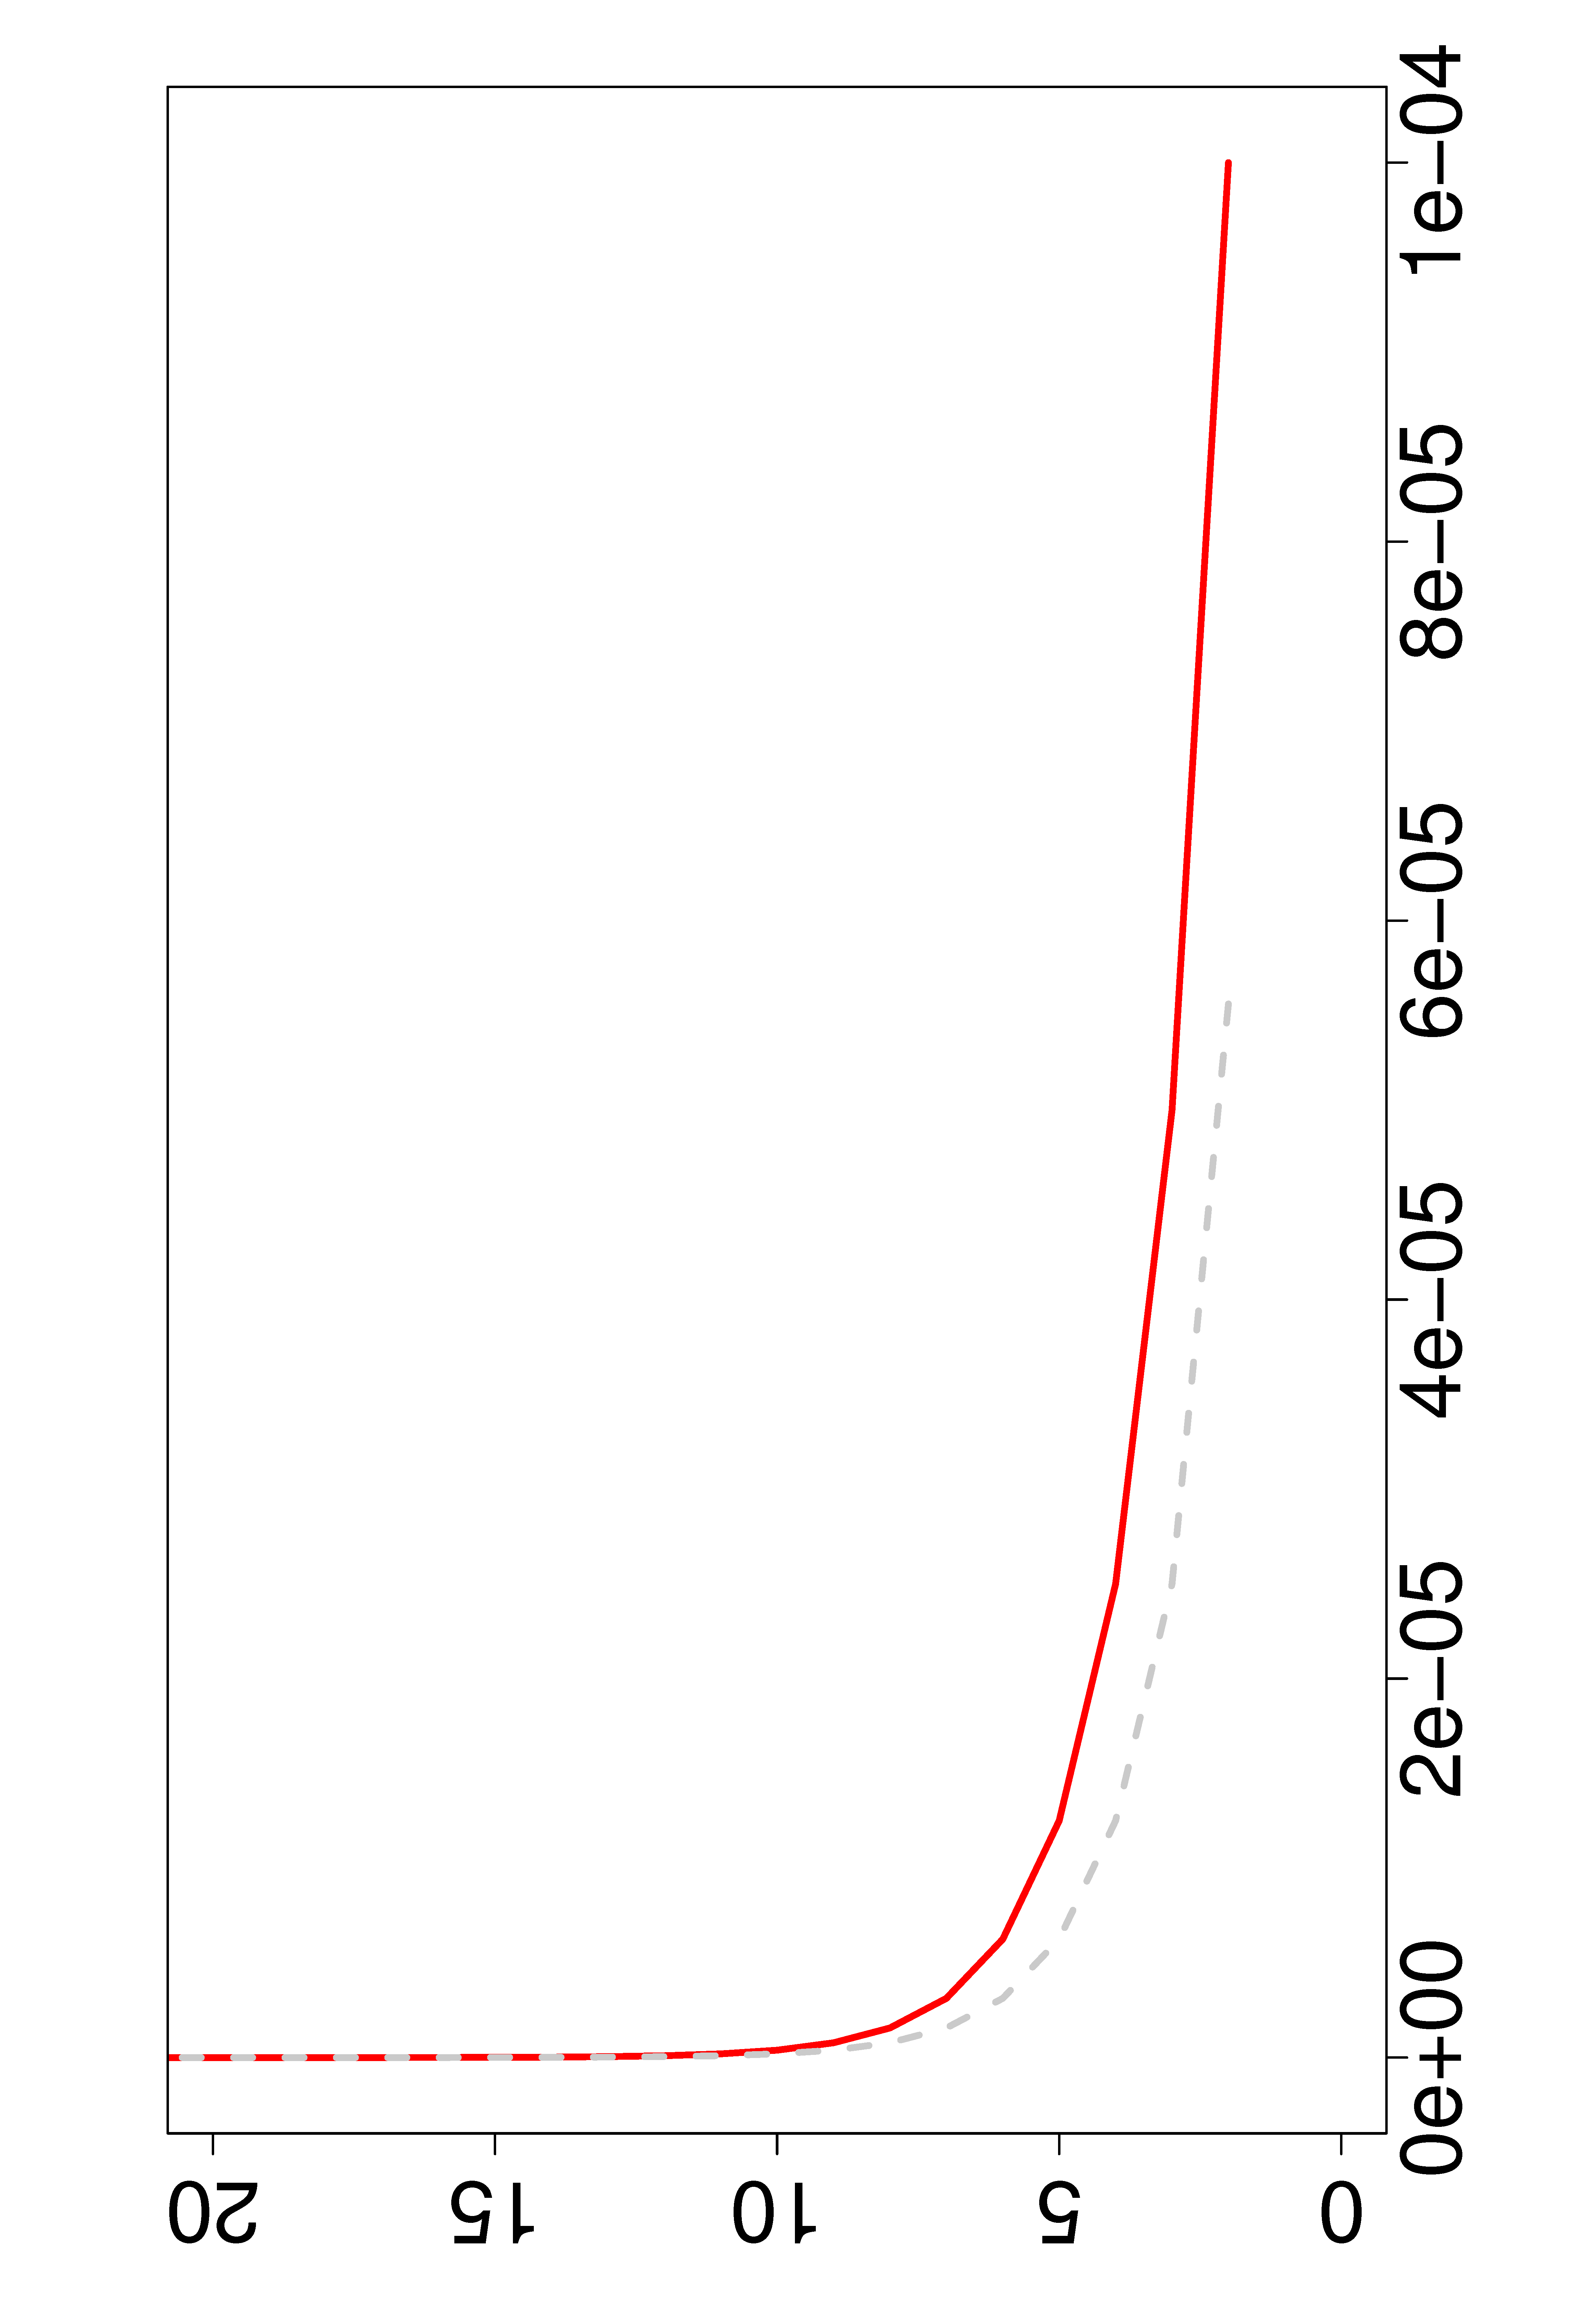
\psfig{file=/RECHERCHE/RUPTURES/MinRegionCont/Res/Abaque-Example.ps,
          width=.4\textheight, height=.4\textwidth, angle=270,
          bbllx=65, bblly=35, bburx=535, bbury=810} \\
        $\ell / L$
      \end{tabular}
    \end{tabular}
  \end{tabular}

  \bigskip\pause
  \paragraph{Aim:} 
  Determine the \emphase{limit couple $(\ell^*, M^*)$} above which the
  alteration can be said significantly recurrent, at level
  (\emphase{at most}) $\alpha$.  
  }

%--------------------------------------------------------------------
\frame{\frametitle{Previous work}
  
  \begin{tabular}{cc}
    \hspace{-0.5cm}
    \begin{tabular}{p{.5\textwidth}}
      The same question is addressed for a \emphase{discrete-time process}
      in \Refer{R \& Stefanov (2009)}\nocite{RoS09}.
      
      \bigskip
      \onslide+<2->{
        \paragraph{Markov chain embedding.} An upper-bound of the
        significance is obtained, based on a Markov
        chain with \\
        $(m+1) + (\ell-2)(m-M+1) + 1$\\
        states.
      }

      \bigskip
      \onslide+<4->{
        \paragraph{NGS cohort studies.} This strategy does not scale to
        \begin{itemize}
        \item NGS data ($\ell = 10^3, L = 10^8$)
        \item and large cohorts ($m = 10^3$ patients)
        \end{itemize}
        }
    \end{tabular}
    &
    \hspace{-.5cm}
    \onslide+<3->{
      \begin{tabular}{p{.5\textwidth}}
        Transition of the embedded MC: \\
        $
        \left(
          \begin{tabular}{c}
            \epsfig{file=../Figures/ExPiR.eps, width=4.5cm, clip=}
          \end{tabular}
        \right)
        $
      \end{tabular}
      }
  \end{tabular}
  }
  

%--------------------------------------------------------------------
\frame{\frametitle{Continous-time Makov model}
  
  Each profile $X_m$ is a continuous time Markov process $X_m =
  \{X_m(t)\}_{0 \leq t \leq L}$:
  $$
  \begin{tabular}{lllll}
    \paragraph{States:} & & $0 = \text{normal}$ & & $1 =
    \text{alteration}$ \\
    \\
    \paragraph{Transition rates:} & & $\lambda : 0 \rightarrow 1$ & &
    $\mu : 1 \rightarrow 0.$ 
  \end{tabular}
  $$

  \bigskip\pause
  \paragraph{Consequence.} \\
  Mean length of \textcolor{darkgreen}{normal regions = $1/\lambda$}
  and \textcolor{red}{altered regions = $1/\mu$}.
  $$
  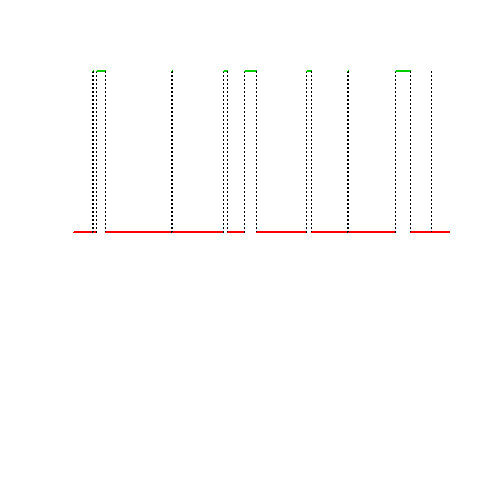
\epsfig{file=../Figures/SingleProfile.ps, clip=,
    width=.2\textheight, height=.8\textwidth, angle=270, bbllx=80,
    bblly=80, bburx=300, bbury=800}
  $$
  }

%--------------------------------------------------------------------
\frame{\frametitle{Event of interest}
  
  We want to calculate the probability of the event $\Ecal$ stating
  that a set of $M$ profiles among the $m$ stay in state 1 during at
  least $\ell$:
  $$
  \Ecal := \left\{
    \begin{array}{ll} 
      \exists (i_1, \dots i_M),&  \forall j=1\dots M, \\
      \exists t \in [\ell; L], & \forall s \in [t-\ell; t]:
    \end{array}
    X_{i_j}(s) = 1\right\}
  $$

  \pause
  \paragraph{Larger event.} The event of interest $\Ecal$ is included
  in a larger event $\Ecal_+$:
  $$
  \Ecal_+ := \left\{
    \begin{array}{ll} 
      \exists t \in [\ell; L], & \forall s \in [t-\ell; t]:
    \end{array}
    \sum_{i=1}^m X_i(s) \geq M\right\}.
  $$
  
  \pause 
  We have
  $$
  \Ecal \subset \Ecal^+ \qquad \Rightarrow \qquad 
  \Pr\{\Ecal\} \leq \Pr\{\Ecal_+\}.
  $$
  and we \emphase{know how to compute the upper bound $\Pr\{\Ecal_+\}$}.
  }
  
%--------------------------------------------------------------------
\section{Birth \& death process}
\frame{\frametitle{Birth \& death process}}
%--------------------------------------------------------------------
\frame{\frametitle{Counting process $X_+$}

  The process
  $$
  \{X_+(t)\}: \qquad X_+(t) := \sum_{i=1}^m X_i(t)
  $$
  counts the number of altered profiles at time $t$. 
  
  \bigskip\pause
  It is a Markovian birth and death process with states $\{0, 1
  \dots, m\}$ and transition rates
  $$
  \begin{array}{llcrcl}
    i \rightarrow i+1 & (\text{'birth' of an alteration}): && \lambda_i &
    = &  (m-i) \times \lambda\\ 
    \\
    i \rightarrow i-1 & (\text{death = back to normal}): && \mu_i & = & i
    \times \mu \\ 
  \end{array}
  $$
  and \emphase{no absorbing state}.
  }

% %--------------------------------------------------------------------
% \frame{\frametitle{Birth \& death processes}

%   \paragraph{Distribution at time $t$.} Denoting $\Rbf$ the transition
%   rate matrix
%   $$
%   \Rbf_{(m+1)\times(m+1)} = \left(\begin{array}{ccccc}
%       \ddots & \ddots & \ddots & & \\
%       & \mu_i & -\lambda_i - \mu_i & \lambda_i & \\
%       & & \ddots & \ddots & \ddots
%     \end{array}\right)
%   $$
%   we have 
%   $$
%   \Pr\{X_+(t+s) = j | X_+(t) = i\} = [\exp(s \Rbf )]_{i, j}.
%   $$

%   \bigskip \pause
%   \paragraph{But} the event $\Ecal_+$  states that $X_+(t)$ stays
%   above $M$ during at least $\ell$ between 0 and $L$ ...
%   ... which has to do with waiting (or \emphase{hitting}) times.
%   }

%--------------------------------------------------------------------
\frame{\frametitle{Waiting for $\Ecal_+$}

  To get $\Ecal_+$ (starting with $X_+(0) = 0$), the process $X_+(t)$
  has to \\
  \begin{tabular}{cc}
    \hspace{-0.5cm}
    \begin{tabular}{p{.5\textwidth}}
      \begin{enumerate}
      \item \onslide+<2->{Reach $M$: \\
          $\emphase{H := Time(0\rightarrow M)},$\\~}
      \item \onslide+<3->{Stay above $M$ more than $\ell$: \\
          $\emphase{A := Time(M \rightarrow M-1)},$\\~}
      \item \onslide+<4->{If it fails ($A < \ell$), reach $M$ again: \\
          $\emphase{B := Time(M-1 \rightarrow M)},$\\~}
      \item \onslide+<5->{Repeat 2 \& 3 until it succeeds ($A \geq
        \ell$), if ever.}
      \end{enumerate}
    \end{tabular}
    &
    \hspace{-1cm}
    \begin{tabular}{p{.6\textwidth}}
      \only<1>{\epsfig{file=../Figures/SumProcess1.ps, clip=,
          width=.7\textheight, height=.5\textwidth, angle=270}\\
        $~$}
      \only<2>{\epsfig{file=../Figures/SumProcess2.ps, clip=,
          width=.7\textheight, height=.5\textwidth, angle=270}\\
        $\qquad H$}
      \only<3>{\epsfig{file=../Figures/SumProcess3.ps, clip=,
          width=.7\textheight, height=.5\textwidth, angle=270}\\
        $\qquad H + A$}
      \only<4>{\epsfig{file=../Figures/SumProcess4.ps, clip=,
          width=.7\textheight, height=.5\textwidth, angle=270}\\
        $\qquad H + A\emphase{\bf ^-} + B$}
      \only<5>{\epsfig{file=../Figures/SumProcess5.ps, clip=,
          width=.7\textheight, height=.5\textwidth, angle=270}\\
        $\qquad H + \sum_{g=1}^G (A_g^- + B_g) + \ell$}
    \end{tabular}
  \end{tabular}
  }
  
%--------------------------------------------------------------------
\frame{\frametitle{Waiting time approach}

  Denoting $\nu^+$ the waiting time
  \begin{eqnarray*}
    \nu^+ & = & \inf_{t \in [\ell; L]}\{t: \forall s \in [t-\ell; t]:
    X_+(s) \geq M\},
  \end{eqnarray*}
  \pause
  we hence have
  $$
  \nu^+ = H + \sum_{g=1}^G (A_g^- + B_g) + \ell
  $$
  \pause where $H$ and $\{B_g\}$ are independent copies of the
  rv's defined above and
  $$
  \begin{array}{rcll}
                                %\begin{eqnarray*}
    \{A_g^-\} \text{ i.i.d } & \overset{\Dcal}{=} & (A | A <
    \ell) & \qquad \text{\emphase{truncated sojourn times} above $M$;}\\
    \pi & = & \Pr\{A \geq \ell\} & \qquad \text{\emphase{success
        probability}}; \\  
    G & \sim & \Gcal(\pi) & \qquad \text{\emphase{number of trials}}. 
                                %\end{eqnarray*}
  \end{array}
  $$

  \pause\bigskip
  Most of all, we have 
  $$
  \emphase{\Pr\{\Ecal_+\} = \Pr\{\nu^+ \leq L\}}.
  $$
  }

%--------------------------------------------------------------------
\section{Laplace transform}
\frame{\frametitle{Laplace transform}}
%--------------------------------------------------------------------
\frame{\frametitle{Laplace transform  and probability generating function}
  For a positive rv $X \sim f$:
  \begin{eqnarray*}
    \text{\paragraph{Probability generating function
        (pgf):}} \qquad \phi_X(s) & = & \Esp(s^X) = \int s^x f(x) \dd x; \\
    \text{\paragraph{Laplace transform (lt):}} \qquad \psi_X(s) & = &
        \Esp(e^{-sX}) = \phi_X(e^{-s}).
  \end{eqnarray*}

  \bigskip \pause
  \paragraph{For independant rv's:}
  \begin{itemize}
  \item Sum:
    $$
    \phi_{X+Y}(s) = \phi_X(s) \phi_Y(s), \qquad \psi_{X+Y}(s) =
    \psi_X(s) \psi_Y(s).
    $$
  \item \pause Sum of a random number of terms: $\{X_1, \dots
    X_{\emphase{G}}\}$ i.i.d.
    $$
    \phi_{X_1+\dots+X_{\emphase{G}}}(s) =
    \phi_{\emphase{G}}[\phi_X(s)], \qquad
    \psi_{X_1+\dots+X_{\emphase{G}}}(s) =
    \phi_{\emphase{G}}[\psi_X(s)].
    $$
  \end{itemize}
  \pause \bigskip
  \paragraph{Laplace transform of the cdf $F$:}
  $$
  \Psi_X(s) = \int e^{-sx} F(x) \dd x = \frac1s \psi_X(s).
  $$
  }

%--------------------------------------------------------------------
\frame{\frametitle{Laplace transform of hitting times}
  
  \paragraph{Hitting time = return time to 0:}
  For a continuous-time Markov process $\{X(t)\}$, we define
  $$
  \tau_k = \inf_{t \leq 0}\{t: X(t) = 0 | X(0) = k\} = Time(k
  \rightarrow 0).
  $$
  \refer{BaS01} provide $\psi_{\tau_k}$ for an arbitrary
  transition rate $\Rbf$.

  \bigskip\pause
  \paragraph{Waiting times $H$, $A$ and $B$} can all be rewritten as
  hitting times.

  \bigskip\pause
  \paragraph{Example for $A$:}
  \begin{itemize}
  \item  Renumber states $\{M-1, M, \dots m\} \rightarrow \{0, 1, \dots,
    m-M+1\}$,
  \item Redefine $\lambda_i = (m-M+1-i) \lambda, \mu_i = (M-1+i)
    \mu$,
  \end{itemize}
  so that
  $$
  A = \tau_1.
  $$
  }

%--------------------------------------------------------------------
\frame{\frametitle{Laplace transform of the waiting time $\nu^+$}

  \paragraph{Reminder.} The pgf of the geometric distribution $\Gcal(\pi)$ is
  $$
  \phi_G(s) = \pi/[1 - (1-\pi)s].
  $$

  \pause
  \paragraph{Playing LEGO.}
  Because $\nu^+$ can be decomposed as
  \begin{eqnarray*}
    \nu^+ & = & H + \sum_{g=1}^G (A_g^- + B_g) + \ell, \pause \\
    \text{we get} \quad
    \psi_{\nu^+}(s) & = & \psi_H(s) \pause
    \phi_G[\psi_{A^- + B}(s)] \pause
    e^{-s\ell} \pause   
    = \frac{\psi_H(s) \pi e^{-s\ell}}{1 - (1-\pi)
      [\psi_{A^-}(s)\psi_{B}(s)]} \pause \\
    \text{that is} \quad
    \Psi_{\nu^+}(s) & = & \emphase{\frac1s
    \frac{\psi_H(s) \pi e^{-s\ell}}{1 - (1-\pi)
      [\psi_{A^-}(s)\psi_{B}(s)]}} \\
  \end{eqnarray*}

  \pause
  \paragraph{Note that} an additional result is required to get
  \emphase{$\psi_{A^-}$}. 
  }

%--------------------------------------------------------------------
\section{Inverting Laplace transforms}
\frame{\frametitle{Inverting Laplace transforms}}
%--------------------------------------------------------------------
\frame{\frametitle{Inverting Laplace transform}
  
  As we are interested in the cdf $F(t) = \Pr\{\nu^+ \leq t\}$, so we
  need to go back
  $$
  \text{from} \qquad \Psi(s) = \int
  e^{-st} F(t) \dd t
  \qquad
  \text{to} \qquad F(t).
  $$
  \pause 
  \refer{AbW06} provide a general framework to achieve this
  inversion based on the following approximation
%   $$
%     F(t) = \frac1{2\pi i t} \int_C \Psi\left(\frac{s}{t}\right)
%     \emphase{e^s} \dd s 
%     \approx \frac1{2\pi i t} \int_C \Psi\left(\frac{s}{t}\right)
%     \emphase{\sum_{k=0}^n \frac{w_k}{a_k - s}} \dd s  
% %     =  \frac1{t} \sum_{k=0}^n w_k \frac1{2\pi i} \int_C
% %     \Psi\left(\frac{s}{t}\right) \frac1{a_k - s} \dd s \\
%     = \frac1{t} \sum_{k=0}^n w_k \Psi\left(\frac{a_k}{t}\right)
%   $$
  \begin{eqnarray*}
    F(t) & = & \frac1{2\pi i t} \int_C \Psi\left(\frac{s}{t}\right)
    \emphase{e^s} \dd s \pause
    \  \approx \  \frac1{2\pi i t} \int_C \Psi\left(\frac{s}{t}\right)
    \emphase{\sum_{k=0}^n \frac{w_k}{a_k - s}} \dd s \pause \\ 
%     & =  & \frac1{t} \sum_{k=0}^n w_k \frac1{2\pi i} \int_C
%     \Psi\left(\frac{s}{t}\right) \frac1{a_k - s} \dd s \\
    & \approx & \frac1{t} \sum_{k=0}^n w_k \Psi\left(\frac{a_k}{t}\right)
  \end{eqnarray*}

  \bigskip\pause
  \paragraph{Several choices} for the weights $w_k$ and the evaluation
  positions $a_k$ are proposed: Gaver-Stehfest, Euler, etc.  
}

%--------------------------------------------------------------------
\frame{\frametitle{Laplace transform inversion in practice}

  \paragraph{Where troubles begin:} Simul/\textcolor{red}{True
    pdf}/\textcolor{blue}{Euler inversion}

  \begin{tabular}{cc}
    $A:$ \epsfig{file =
      ../../MinRegionCont/Res/Simul-m50-L1-M7-lambda5-mu100-A-pdf.ps,
      clip=, width=.25\textwidth, angle=270, bbllx=60, bblly=40,
      bburx=540, bbury=780}
    &
    $B:$ \epsfig{file =
      ../../MinRegionCont/Res/Simul-m50-L1-M7-lambda5-mu100-B-pdf.ps,
      clip=, width=.25\textwidth, angle=270, bbllx=60, bblly=40,
    bburx=540, bbury=780} 
    \\
    $H:$ \epsfig{file =
      ../../MinRegionCont/Res/Simul-m50-L1-M7-lambda5-mu100-H-pdf.ps,
      clip=, width=.25\textwidth, angle=270, bbllx=60, bblly=40,
    bburx=540, bbury=780}
    &
    $A^-:$ \epsfig{file =
      ../../MinRegionCont/Res/Simul-m50-L1-M7-lambda5-mu100-Ainf-pdf.ps,
      clip=, width=.25\textwidth, angle=270, bbllx=60, bblly=40,
    bburx=540, bbury=780}   
  \end{tabular}
  }

% --------------------------------------------------------------------
% \frame{\frametitle{Laplace transform inversion in practice (cont'd)}

%   \paragraph{Where troubles begin:} Simul/\textcolor{red}{True
%     cdf}/\textcolor{blue}{Euler inversion}

%   \begin{tabular}{cc}
%     $A:$ \epsfig{file =
%       ../../MinRegionCont/Res/Simul-m50-L1-M7-lambda5-mu100-A-cdf.ps,
%       clip=, width=.25\textwidth, angle=270, bbllx=60, bblly=40,
%       bburx=540, bbury=780}
%     &
%     $B:$ \epsfig{file =
%       ../../MinRegionCont/Res/Simul-m50-L1-M7-lambda5-mu100-B-cdf.ps,
%       clip=, width=.25\textwidth, angle=270, bbllx=60, bblly=40,
%     bburx=540, bbury=780} 
%     \\
%     $H:$ \epsfig{file =
%       ../../MinRegionCont/Res/Simul-m50-L1-M7-lambda5-mu100-H-cdf.ps,
%       clip=, width=.25\textwidth, angle=270, bbllx=60, bblly=40,
%     bburx=540, bbury=780}
%     &
%     $A^-:$ \epsfig{file =
%       ../../MinRegionCont/Res/Simul-m50-L1-M7-lambda5-mu100-Ainf-cdf.ps,
%       clip=, width=.25\textwidth, angle=270, bbllx=60, bblly=40,
%     bburx=540, bbury=780}   
%   \end{tabular}
%   }

%--------------------------------------------------------------------
\frame{\frametitle{A lower bound}
  
  \paragraph{A smaller event $\Ecal^-$.} Denoting
  $$
  \Ecal^- = \left\{\begin{array}{l}
      \exists t \leq L-\ell: X_+(t) = M, \\
      \forall j: X_j(t) = M,
    \end{array}
    \forall s \in [t; t+\ell]: X_j(s) \geq M \right\},
  $$
  we have
  $$
  \Ecal^- \subset \Ecal \qquad \Rightarrow \qquad \Pr\{\Ecal^-\} \leq
  \Pr\{\Ecal\}.
  $$
  
  \pause
  \paragraph{Furthermore}
  \begin{eqnarray*}
    \Pr\{\Ecal^-\} & = & \Pr\{H \leq L-\ell\} \Pr\{\text{None of the $M$
      alterations ends before $\ell$}\} \pause \\
    & = & \Pr\{H \leq L-\ell\} \exp(-M \mu \ell)
  \end{eqnarray*}
  
  \pause
  \paragraph{Accuracy of the bounds:} Can be evaluated through the
  difference between $\Pr\{\Ecal^+\}$ and $\Pr\{\Ecal^-\}$. 
  
  }

%--------------------------------------------------------------------
\section{Results}
\frame{\frametitle{Results}}

%--------------------------------------------------------------------
\frame{\frametitle{Results: Several scenarios}
  \paragraph{Breast cancer data:}
  \begin{itemize}
  \item The chromosome length is about $L \simeq 10^8$nt;
  \item The alteration lengths range from $10^3$ to $10^6$nt
    (i.e. $10^{-5}L$ to $10^{-2}L$);
  \item There are between 1 and 100 alterations per individual
    chromosome.
  \end{itemize}

  \bigskip\pause
  This observation provide typical valued for $\lambda$ and $\mu$ via
  \begin{eqnarray*}
  \text{Mean number of alterations} & = & L \left(\frac1{\lambda} +
  \frac1{\mu}\right)^{-1}, \\  
  \text{Mean alteration length} & = & 1/\mu.
  \end{eqnarray*}
  }

%--------------------------------------------------------------------
\frame{\frametitle{Significance curves}

  \begin{tabular}{ccc}
    \paragraph{$\begin{array}{l}
        m = 100 \\
        \alpha = 1\%
      \end{array}$}
    & Short alter.: $10^{-5} L$ & Long alter.: $10^{-3} L$ \\
    \begin{tabular}{l}
      Rare \\
      alterations \\
      (1/chrom.)
    \end{tabular}    
    &
    \begin{tabular}{c}
      \epsfig{file =
        ../../MinRegionCont/Res/Abaque-UpperLower-m100-L1-lambda1-mu1e+05.ps, 
        width=0.2\textwidth, clip=, angle=270, bbllx=65, bblly=35,
      bburx=535, bbury=810}
    \end{tabular}    
    &
    \begin{tabular}{c}
      \epsfig{file =
        ../../MinRegionCont/Res/Abaque-UpperLower-m100-L1-lambda1-mu1000.ps, 
        width=0.2\textwidth, clip=, angle=270, bbllx=65, bblly=35,
      bburx=535, bbury=810}
    \end{tabular}    
    \\
    \begin{tabular}{l}
      Numerous \\
      alterations \\
      (100/chrom.)
    \end{tabular}    
    &
    \begin{tabular}{c}
      \epsfig{file =
        ../../MinRegionCont/Res/Abaque-UpperLower-m100-L1-lambda100-mu1e+05.ps, 
        width=0.2\textwidth, clip=, angle=270, bbllx=65, bblly=35,
      bburx=535, bbury=810}
    \end{tabular}    
    &
    \begin{tabular}{c}
      \epsfig{file =
        ../../MinRegionCont/Res/Abaque-UpperLower-m100-L1-lambda111-mu1000.ps, 
        width=0.2\textwidth, clip=, angle=270, bbllx=65, bblly=35,
      bburx=535, bbury=810}
    \end{tabular}    
  \end{tabular}    
  }

%--------------------------------------------------------------------
\frame{\frametitle{Further work}

  \paragraph{Assess the numerical accuracy} of the Laplace transform
  inversion. 

  \bigskip\pause
  \paragraph{Improve the lower bound.} ...

  \bigskip\pause
  \paragraph{Consider other modelling} that allows us to consider larger
  cohort size, e.g. $m = 10^3, 10^4$. \\
  \ra Continuous space state $[0; m]$?  

  \bigskip\pause
  \paragraph{Some references.}
  {\scriptsize
    \bibliography{/Biblio/ARC,/Biblio/AST,/Biblio/SSB}
    \bibliographystyle{/Latex/astats}
                                %\bibliographystyle{plain}
    }
  }

%--------------------------------------------------------------------

%--------------------------------------------------------------------
%--------------------------------------------------------------------
\end{document}
%--------------------------------------------------------------------
%--------------------------------------------------------------------

%--------------------------------------------------------------------
\frame{\frametitle{}
  }


  \vspace{-0.5cm}
  \begin{tabular}{cc}
    \hspace{-0.5cm}
    \begin{tabular}{p{.5\textwidth}}
    \end{tabular}
    &
    \hspace{-1cm}
    \begin{tabular}{p{.5\textwidth}}
    \end{tabular}
  \end{tabular}
